\chapter{The TFSM and Activity Languages}
\label{ap:languages}

\todo{To add the description of Activity language}

To illustrate the approach, we introduce a simple state-based language named Timed Finite State Machine (TFSM) and its behavioral interface; a state machine language augmented with timed transitions (see Figure~\ref{fig:tfsmmm}). The metamodel describes the abstract syntax of the TFSM language (see Figure~\ref{fig:tfsmmm}). A \emph{System} is composed of \emph{TFSMs}, global \emph{FSMEvents} and global \emph{FSMClocks}. Each \emph{TFSM} is composed of \emph{States}. Each state can be the source of outgoing guarded \emph{Transitions}. A guard can be specified either by the reception of an \emph{FSMEvent} (\emph{EventGuard}) or by a duration relative to the entry time in the source state of the transition (\emph{TemporalGuard}). When fired, transitions generate a set of simultaneous \emph{FSMEvent} occurrences.

The TFSM language defines the following \dse: \emph{entering} and \emph{leaving} a state, \emph{firing} a transition, the occurrences (\emph{occurs}) of a FSMEvent and the \emph{ticks} of a FSMClock (see at the top of Figure~\ref{fig:tfsmmm}). These \dse are part of the language behavioral interface of TFSM. \dse are defined by using a specific language named \ecl (standing for Event Constraint Language~\cite{ECL}) which is an extension of OCL~\cite{omgocl2} with events. \ecl takes benefits from the OCL query language and its possibility to augment an abstract syntax with additional attributes (without any side effects). Consequently by using \ecl, it is possible to augment \as metaclasses and add \dse. A partial \ecl specification of TFSM is shown in Listing~\ref{fig:tfsmmmecl} where the \dse \textit{entering} and \textit{leaving} are defined in the context of State (Listing~\ref{fig:tfsmmmecl}: line 6) while \textit{occurs} is defined in the context of FSMEvent (Listing~\ref{fig:tfsmmmecl}: line 4). When a metaclass is instantiated, the corresponding \dse are instantiated; \eg for each instance of the metaclass \emph{State}, \dse \textit{entering} is instantiated. Each instance of \dse is a \mse. In the case of TFSM, since two States are instantiated (\emph{S1} and \emph{S2}), there are two \mse of \textit{entering}: \textit{S1\_entering} and \textit{S2\_entering}. All \mse are part of the model behavioral interface. 
%\eject
\begin{figure}
	\begin{center}
		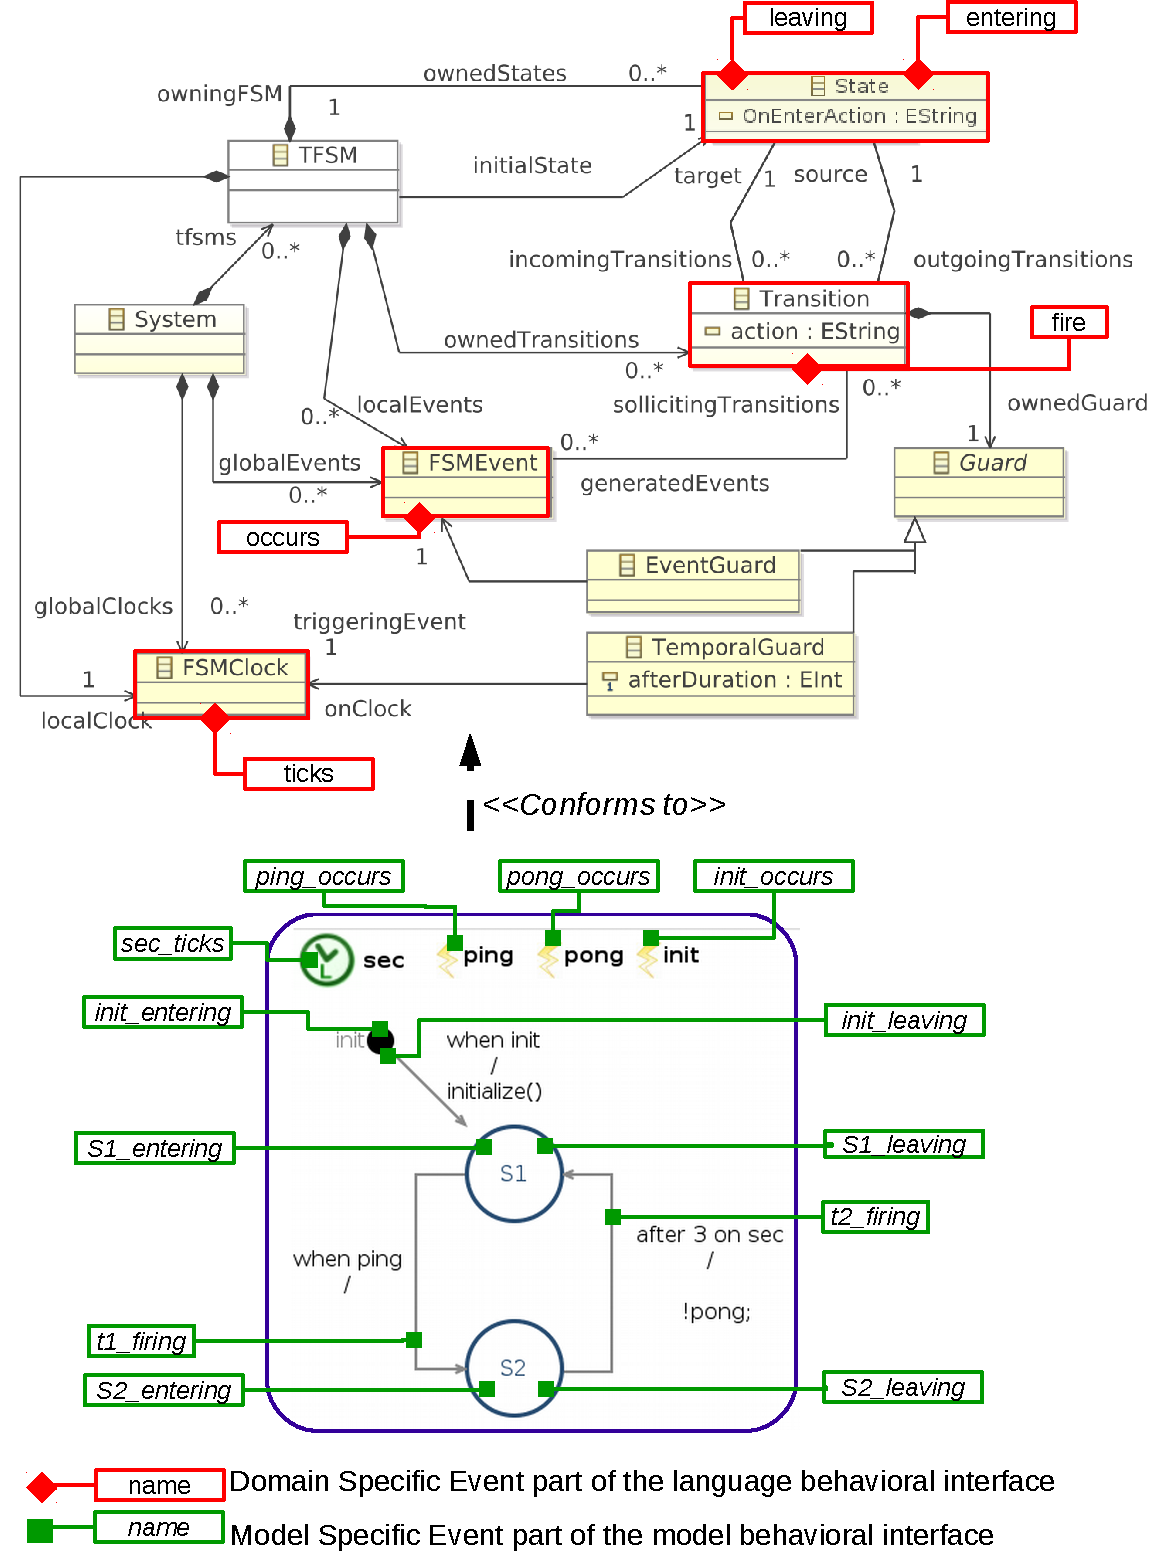
\includegraphics[width=1\textwidth]{appendix/figs/tfsmlang}
		\caption{(At the top) The TFSM metamodel with its language behavioral interface. (At the bottom)  a TFSM model with its model behavioral interface}
		\label{fig:tfsmmm}
	\end{center}
\end{figure}

\begin{lstlisting}[language=ecl,
caption={Partial \ecl specification of TFSM},
label={fig:tfsmmmecl}, 
basicstyle=\scriptsize\ttfamily, backgroundcolor=\color{LGrey}, numbers=left, xleftmargin=3pt]
package tfsm
context FSMClock
def: ticks : Event = self
context FSMEvent
def: occurs : Event = self
context State
def : entering : Event = self
def : leaving : Event = self
\end{lstlisting}


Before going into the example, we briefly present the language behavioral interface of the fUML language partially shown in  Listing~\ref{fig:eclfuml}. For each \emph{Activity} two \dse are defined: \emph{startActivity} and \emph{finishActivity}, to identify respectively the starting and finishing instants of the activity. Similarly, Two \dse are defined for each \emph{Action}: \emph{startAction} and \emph{finishAction}, to identify the starting and the finishing of an Action. These \dse, part of the fUML language behavioral interface, are used throughout this section to specify the coordination operators.

\begin{lstlisting}[language=ecl,
caption={Partial \ecl specification of Activity Diagram},
label={fig:eclfuml}, 
basicstyle=\scriptsize\ttfamily, backgroundcolor=\color{LGrey}, numbers=left, xleftmargin=3pt, belowskip=-0.4em]
package uml
context Activity
def: startActivity : Event = self
def: finishActivity: Event = self
context Action
def : startAction : Event = self
def : finishAction : Event = self
\end{lstlisting}

\begin{figure}
	\begin{center}
		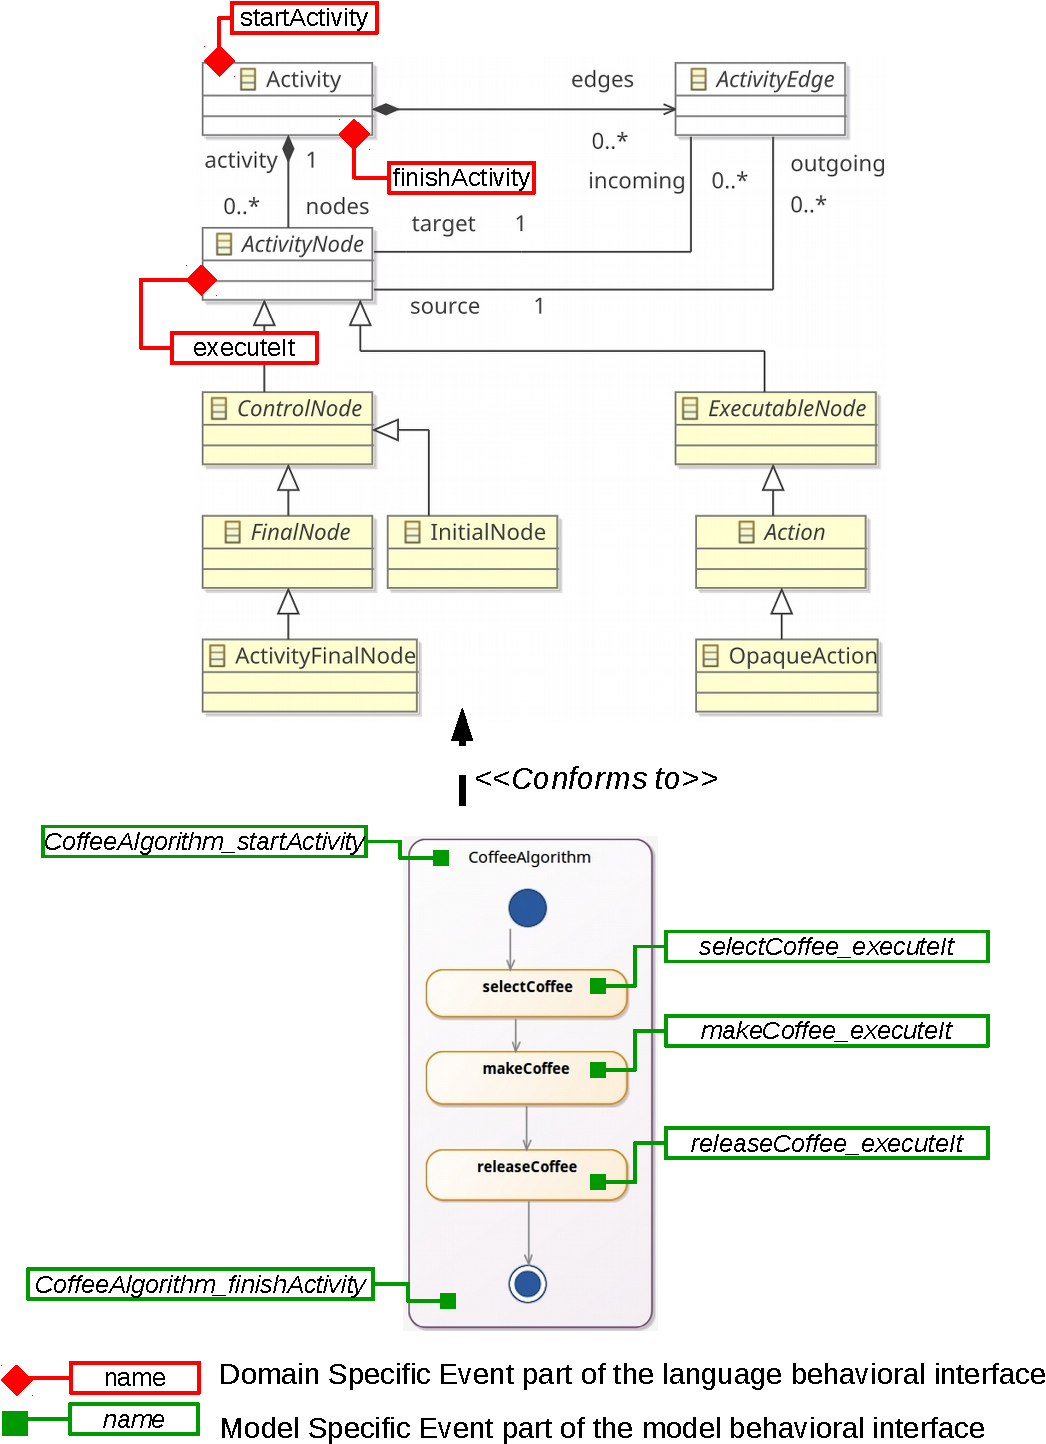
\includegraphics[width=1\textwidth]{appendix/figs/activitylang}
		\caption{(At the top) The Activity metamodel with its language behavioral interface. (At the bottom) an Activity model with its model behavioral interface}
		\label{fig:tfsmmm}
	\end{center}
\end{figure}
